\section{Introduction}\label{sec:intro}

\begin{figure*}
    \centering
    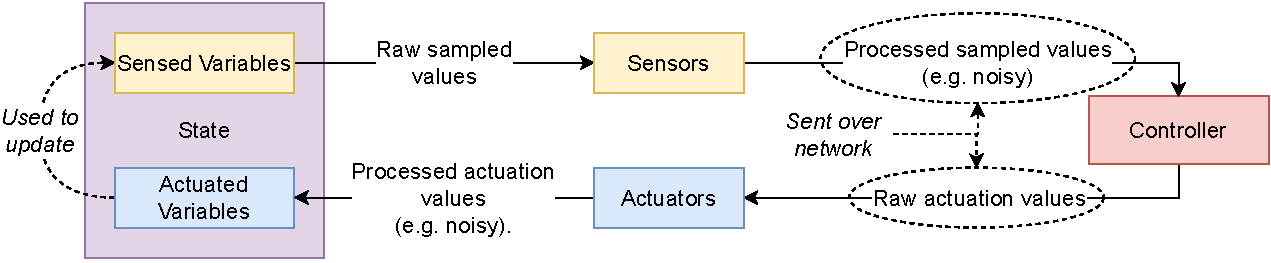
\includegraphics[width=.8\textwidth]{publications/2022CLEAVE/images/CLEAVE_NCS_structure}
    \caption{
        Structure of an emulated \acl*{NCS} in \acs*{CLEAVE}.
    }\label{fig:cleave:ncs:struct}
\end{figure*}

The number and applications of \acp{CPS}~\cite{Rajkumar2010CPS} --- i.e.\ systems in which a real, physical mechanism is controlled by a computer --- have exploded in recent years.
However, this rapid increase in adoption has mostly been limited to industrial contexts.
Although \acp{CPS} present huge opportunities for all facets of society, they have yet to reach our daily lives in any relevant scale due to their stringent operational requirements.
This is about to change, however, as with the advent of novel wireless communication technologies as well as networking paradigms, such as cellular 5G and edge computing~\cite{Satya2017Emergence}, consumer-grade \acp{CPS} will be made possible.
These technologies meet two key requirements of \acp{CPS}: real-time capabilities (through extremely low end-to-end latencies), and context- and locality-awareness, and will most likely become the backbone of \gls{CPS} in the future.

\acp{NCS}~\cite{Gupta2010NCSOverview}, a type of \gls{CPS} wherein multiple networked actuators and sensors form a part of the same automatic control system will benefit from the adoption of these technologies.
Depending on the physical system being controlled, \acp{NCS} can have stringent timing and reliability requirements for communication that conventional cloud paradigms and cellular networks cannot meet~\cite{Wan2020Efficient}.
This necessitates sophisticated tools for the performance evaluation of future system architectures, as well as novel NCS design paradigm.

%Due to their potential advantages for industrial and commercial settings, there exist works~\cite{Zhang2016Survey} dedicated to the modelling and performance characterization of \acp{NCS}, improving NCSs by distributing control functions across networks, facilitating centralized coordination, control, and monitoring.

One the one hand, related literature in \acp{NCS} leverages to a large extent theoretical models, at the price of being able to capture networked systems effects only on a coarse level. 
%follows a theoretical approach, and only a small fraction of it deals with experimental studies.
On the other, there exist several approaches when considering experimental methodologies. 
%A number of works concerning \acp{NCS} deal with experimental studies.
%\acp{NCS} have an inherently inter-domain nature intertwining knowledge from the fields of communications, computing, and control theory in ways that cannot be studied in isolation, leading to various different approaches to such studies.
One such approach uses setups in which the complete system is built on top of real hardware.
This approach is employed in the works of Baumann \emph{et al.}~\cite{Baumann2018LowPower} and Cuenca \emph{et al.}~\cite{Cuenca2019UAV}; in both of these, the authors implement their approach on physical testbeds.
Conversely, other studies choose to instead use completely \emph{simulated} \gls{NCS} setups.
The authors in\ \cite{Ma2019DynamicSched} have opted for such an approach.
These studies often employ combinations of physical and network simulation tools trying to capture the complex dynamics of \acp{NCS}.
Finally, some experimental studies instead employ \emph{virtualized} approaches, in which either
\begin{enumerate*}[itemjoin={{; }}, itemjoin*={{; or }}]
    \item a real network interacts with a simulated or emulated control system~\cite{Wang2020VoltageControl}
    \item a simulated network interacts with a real control system~\cite{Natale2004InvPendEthernet}.
\end{enumerate*}

As evidenced above, experimental research in \acp{NCS} includes varied heterogeneous hardware and software platforms, methodologies and key performance indicators.
This, in turn, leads to hardware, software, and methodology fragmentation, as different studies tend to prefer approaches more favored in their respective communities.
Furthermore, existing studies tend to focus on individual aspects and components of a system, thus producing results which do not provide a complete image of the \gls{NCS}.
This has caused a gap in knowledge pertaining to the reproducibility and comparison of experimental studies on these systems.

Zoppi \emph{et al.}~\cite{Zoppi2020NCSBench} made the first (and to the best of our knowledge, the only) attempt at tackling this challenge in their work.
In their work, they proposed a platform called NCSBench, to be used for reproducible benchmarking in NCS.\ 
Their methodology utilizes joint knowledge of control, computation, and communication. 
In their work various architectural elements and the corresponding delays associated with the NCS are modelled. 
Multiple experimental parameters and certain observable key performance indicators are defined and utilized in the implementation. 
This work however utilizes a physical LEGO\textregistered{}\ Mindstorms EV3 Core Set\texttrademark{}\  based plant for the implementation, preventing instantaneous changes in plant characteristics and component parametrizations.
Furthermore, relying on physical objects like an inverted pendulum limits scalability of the experimentation in practice. 

We overcome this issue by proposing a completely virtual plant allowing for unparalleled flexibility in changing the plant model and characteristic features of the experiments.
In this paper, we present the first fully-software-based framework for scalable and repeatable benchmarking of edge-native \gls{NCS}.
As edge computing begins being adopted by industry, more and more variations have begun to appear in literature.
``Near'', ``far'', ``core'', and ``telco'' edge describe variations of the original concept and are becoming ubiquitous in new research.
While the core idea of edge computing is widely accepted as fundamental for pervasive \acp{NCS} in general, understanding the strengths and weaknesses of such different edge concepts is of paramount importance.

Our framework, \gls{CLEAVE}, aims to simplify the repeatable and scalable benchmarking of such systems.
It is fully virtualized, inspired by our previous work on benchmarking human-in-the-loop applications on the edge~\cite{Olguin2019EdgeDroid}.
The tool consists of a benchmarking framework and software development kit for the development of emulated physical systems and softwarized controllers.
These virtual \acp{NCS} can then be deployed on real networks for reparametrizable, repeatable, and reproducible benchmarking of the complete system.

\gls{CLEAVE} is built using \emph{Python 3.8}, making it highly extensible and able to harness the multitude of already existing user libraries.
It is furthermore compatible with container technologies such as \emph{Docker}\footnote{Docker Engine: \url{https://www.docker.com/}}, making it suitable for automated deployment, scaling, and benchmarking on industry-standard edge setups using container orchestration solutions.

The rest of this paper is structured as follows.
\cref{sec:approach} presents the design principles and implementation of the framework.
In \cref{sec:experiments}, we present a use case scenario which validates the utility, flexibility, and repeatability of \gls{CLEAVE}.
Finally, in \cref{sec:conclusion} we conclude this work.